\documentclass[10pt]{article}

%Math
\usepackage{amsmath}
\usepackage{amsfonts}
\usepackage{amssymb}
\usepackage{amsthm}
\usepackage{ulem}
\usepackage{stmaryrd} %f\UTF{00FC}r Blitz!

%PageStyle
\usepackage[ngerman]{babel} % deutsche Silbentrennung
\usepackage[utf8]{inputenc} 
\usepackage{fancyhdr, graphicx}
\usepackage[scaled=0.92]{helvet}
\usepackage{enumitem}
\usepackage{parskip}
\usepackage[a4paper,top=2cm]{geometry}
\setlength{\textwidth}{17cm}
\setlength{\oddsidemargin}{-0.5cm}


% Shortcommands
\newcommand{\Bold}[1]{\textbf{#1}} %Boldface
\newcommand{\Kursiv}[1]{\textit{#1}} %Italic
\newcommand{\T}[1]{\text{#1}} %Textmode
\newcommand{\Nicht}[1]{\T{\sout{$ #1 $}}} %Streicht Shit durch

%Arrows
\newcommand{\lra}{\leftrightarrow} 
\newcommand{\ra}{\rightarrow}
\newcommand{\la}{\leftarrow}
\newcommand{\lral}{\longleftrightarrow}
\newcommand{\ral}{\longrightarrow}
\newcommand{\lal}{\longleftarrow}
\newcommand{\Lra}{\Leftrightarrow}
\newcommand{\Ra}{\Rightarrow}
\newcommand{\La}{\Leftarrow}
\newcommand{\Lral}{\Longleftrightarrow}
\newcommand{\Ral}{\Longrightarrow}
\newcommand{\Lal}{\Longleftarrow}

% Code listenings
\usepackage{color}
\usepackage{xcolor}
\usepackage{listings}
\usepackage{caption}
\DeclareCaptionFont{white}{\color{white}}
\DeclareCaptionFormat{listing}{\colorbox{gray}{\parbox{\textwidth}{#1#2#3}}}
\captionsetup[lstlisting]{format=listing,labelfont=white,textfont=white}
\lstdefinestyle{JavaStyle}{
 language=Java,
 basicstyle=\footnotesize\ttfamily, % Standardschrift
 numbers=left,               % Ort der Zeilennummern
 numberstyle=\tiny,          % Stil der Zeilennummern
 stepnumber=5,              % Abstand zwischen den Zeilennummern
 numbersep=5pt,              % Abstand der Nummern zum Text
 tabsize=2,                  % Groesse von Tabs
 extendedchars=true,         %
 breaklines=true,            % Zeilen werden Umgebrochen
 frame=b,         
 %commentstyle=\itshape\color{LightLime}, Was isch das? O_o
 %keywordstyle=\bfseries\color{DarkPurple}, und das O_o
 basicstyle=\footnotesize\ttfamily,
 stringstyle=\color[RGB]{42,0,255}\ttfamily, % Farbe der String
 keywordstyle=\color[RGB]{127,0,85}\ttfamily, % Farbe der Keywords
 commentstyle=\color[RGB]{63,127,95}\ttfamily, % Farbe des Kommentars
 showspaces=false,           % Leerzeichen anzeigen ?
 showtabs=false,             % Tabs anzeigen ?
 xleftmargin=17pt,
 framexleftmargin=17pt,
 framexrightmargin=5pt,
 framexbottommargin=4pt,
 showstringspaces=false      % Leerzeichen in Strings anzeigen ?        
}

%Config
\renewcommand{\headrulewidth}{0pt}
\setlength{\headheight}{15.2pt}

%Metadata
\title{
	\vspace{5cm}
	Uebung 5 Dokumentation
}
\author{Jonas Schwammberger}
\date{5. Semester (HS 2013)}


% hier beginnt das Dokument
\begin{document}

% Titelbild
\maketitle
\thispagestyle{fancy}

\newpage

% Inhaltsverzeichnis
%\pagenumbering{Roman}
%\tableofcontents	  	


\newpage
\setcounter{page}{1}
\pagenumbering{arabic}

% Inhalt Start


\section{Algorithmus für die Konvexe Hülle}
Für die Berechnung der Konvexen Hülle standen zwei Algorithmen zur Verfügung. Der Algorithmus von Graham und von Jarvis March. Welcher Algorithmus (O(n log n) versus O(n*m)) besser ist, hängt vom Eingabeverhalten des Benutzers ab. Da ich zum durchschnittlichen Verhalten keine Daten habe wurde Graham ausgewählt. Der Algorithmus von Graham wurde aus interesse von mir selber implementiert und modifiziert.

\subsection{Modifikation}
Die Modifikation beschränkt sich darauf, dass nach dem Abbrechen der Hauptschleife nochmals eine isConvex() Prüfung mit Punkt $P_{0}$, PN und PN-1. Im falle das PN auf der Strecke zwischen $P_{0}$ und PN-1 ist PN nicht in der minimalen konvexen Hülle. Dies prüft der Algorithmus von Graham nicht, deshalb wurde diese Modifikation vorgenommen.

\section{Algorithmus für die Berechnung des minimalen Rechtecks}
Die Algorithmus startet mit dem minimalen achsenparalellen Rechteck der Convexen Hülle. Nun werden alle Strecken des Rechtecks um den Berührungspunkt gedreht, bis sie sich eine Strecke einen neuen Punkt der Konvexen Hülle berührt. Bei jede Berührung ist ein Kandidat für das minimale Rechteck. Wenn sich die Strecke mit einem neuen Punkt berührt hat, wird sie nun um den neuen Berührungspunkt weiter gedreht. Alle Strecken werden maximal um 90$^\circ$ gedreht, dann ist die Ausgangslage erreicht und das minimale Rechteck mindestens ein Mal besucht.

Somit hat dieser Algorithmus einen Worst-Case von O(n). Er kann schneller abbrechen falls die Figur kleine Innenwinkel aufweist.

Der Algorithmus braucht mindestens vier Punkte, deshalb muss beim Input von drei Punkten eine Sonderbehandlung durchgeführt werden.

\subsection{Sonderbehandlung bei drei Punkten}
Bei drei Punkten muss man nur das minimale Rechteck eines Dreiecks finden. Das minimale Rechteck liegt immer mit einer seite an der längsten Seite des Dreiecks.

\subsection{Implementation}

\subsection{Nachteile}
Der grösste Nachteil dieser Implementierung ist, dass für die Drehung Floating Point Datentypen verwendet werden müssen. Bei der Konvertierung von Floating Point zu Integer kommen oft Fehler von +-1 vor, welches auf der Graphik sofort Sichtbar ist.
\begin{figure} [h!]

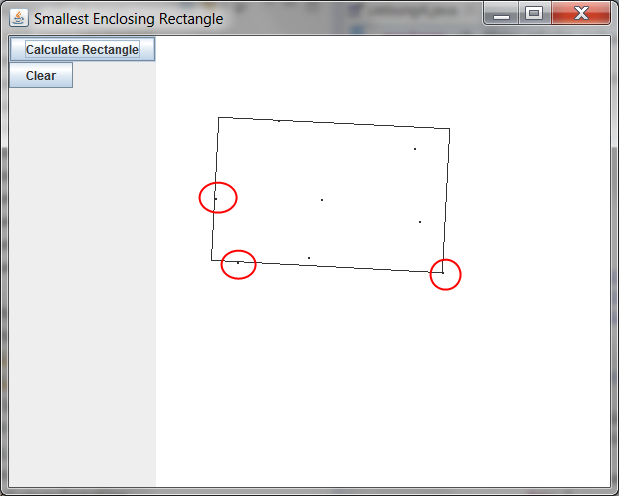
\includegraphics[scale= 0.75]{screenshot.png}
\caption{Fehler in der Graphik}
\end{figure}

% Inhalt Ende 
\end{document} 